% Tento soubor nahraďte vlastním souborem s obsahem práce.
%=========================================================================
% Autoři: Michal Bidlo, Bohuslav Křena, Jaroslav Dytrych, Petr Veigend a Adam Herout 2019

% Pro kompilaci po částech (viz projekt.tex), nutno odkomentovat a upravit
%\documentclass[../projekt.tex]{subfiles}
%\begin{document}


\newcommand{\highlight}[1]{\colorbox{purple}{\color{white}#1}}
\newcommand{\todoimage}[2]{
    \begin{figure}[H]
        \centering
        
\includegraphics[#1]{obrazky-figures/placeholder.pdf}
        \caption{\textbf{#2} \todo{popisek}}
    \end{figure}
}


% \renewcommand{\dummyShortText}[1][1]{}
% \renewcommand{\dummyText}[1][1]{}
% \renewcommand{\DummyText}{}
% \renewcommand{\todoimage}[2]{}


%*********************************************************************************
%                                    1 ÚVOD
%*********************************************************************************
\chapter{Úvod}

\dummyText

\dummyText[2]

\dummyShortText[15]

%*********************************************************************************




%*********************************************************************************
%                                 2 TYPOGRAFIE
%*********************************************************************************
\chapter{Rychlokurz typografie}


%*********************************************************************************




%*********************************************************************************
%                                2 ČASTÉ CHYBY
%*********************************************************************************
\chapter{Často vyskytované chyby v~diplomových pracích}
\cite{Ctenar_12_2015}

\dummyShortText[6]

\dummyText


%#######################    2.1 Přetečení obsahu za okraj    #######################
\section{Přetečení obsahu za okraj}
Přetečení textu za okraj se nejčastěji vyskytuje, když student píše svou diplomovou
práci s~pomocí jazyka {\LaTeX}. Obvykle je to způsobeno tím, že program nedokáže
automaticky zalomit slovo na konci řádku, jak je ukázáno na
obrázku~\ref{pic_overflow}. Toto lze opravit napověděním možného
zalomení nebo přeformulováním věty, kde se daná chyba vyskytuje.
Další typ této chyby je přetečení obrázku za okraj,
který se nestává tak často, ale lze jej udělat v~několika textových editorech.

\begin{figure}[H]
    \label{pic_overflow}
    \centering
    %
\includegraphics[width=\linewidth,height=1.7in]{obrazky-figures/placeholder.pdf}
    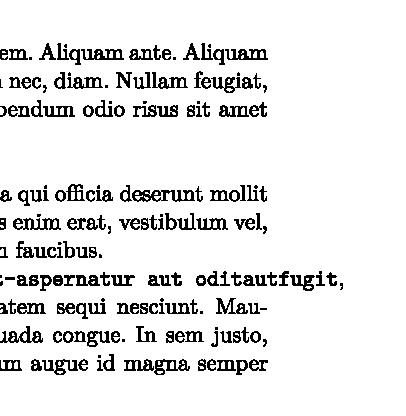
\includegraphics{obrazky-figures/overflow.pdf}
    \caption{\textbf{Ukázka přetečení za okraj.} \todo{popisek}}
\end{figure}


%#######################    2.2 Spojovník x pomlčka    #######################
\section{Špatné použití spojovníku}
Špatné používání spojovníku je chyba, která se vyskytuje nejen v~diplomových
pracích. Spojovník (-) je graficky velmi podobný pomlčce (--), ale významově
se značně liší. Pravidla pro psaní těchto znaků, uvedena v~internetové příručce
Ústavu pro jazyk český~\cite{Ustav_pro_jazyk_cesky},
říkají, že spojovník se píše bez mezer mezi výrazy, které spojuje. Výjimkou
je, naznačuje-li spojovník neúplné slovo. Obecně tedy v~češtině tento znak
užíváme tehdy, chceme-li vyjádřit, že jím spojené výrazy tvoří těsný významový
celek. Pomlčka se oproti spojovníku využívá pro oddělování částí projevu,
vyjádření rozsahu, vztahu nebo vyznačení přestávky v~řeči, pro uvození
přímé řeči a~pro vyjádření celého čísla při psaní peněžních částek.
Oddělujeme ji z~obou stran mezerami. Komplikovanější situace nastane pouze
tehdy, když je toto znaménko použito ve funkci výrazů a, až, od, do nebo proti.
Spojovník (-) i~pomlčka (--) bývají často zaměňovány se znaménkem minus ($-$),
to však má též své grafické i~významové odlišnosti.
V~knize~\cite{Pruvodce_tvorbou_dokumentu} je vysvětleno, že znak minus má stejnou
šíři i~umístění jako znak plus. Znak minus se používá ve dvou významech, a to
pro označení záporné hodnoty, nebo pro označení operace odčítání. Sazba se v~obou
případech liší: pro označení záporné hodnoty se znak minus a~následující
operand píše bez mezery, pro psaní minus jako odčítání se však mezera uvádí
z~obou stran tohoto znaménka. Internetové příručka Ústavu pro jazyk
český~\cite{Ustav_pro_jazyk_cesky} však uvádí, že je v~korespondenci dovoleno
znak minus ($-$) nahradit pomlčkou (--).

Podle článku~\cite{Zaklady_typografie:Slezakova} se tato chyba (naznačena na
obrázku~\ref{TODO:}) vyskytuje v~textu kvůli absenci znaku pomlčky na klávesnici.
Místo znaku pomlčky, který je pravděpodobně častěji potřebný při psaní textu,
se na klávesnici vyskytuje právě znak spojovníku. I~když nyní už spousta
textových editorů dokáže automaticky nahradit spojovník za pomlčku, tato náhrada
nemusí být stoprocentní. V~programu {\LaTeX} se spojovník zapíše přímo
z~klávesnice jako \verb|-|,
pomlčku je možno zapsat pomocí dvou spojovníků \verb|--| a~znaménko minus je
zapsáno jako spojovník v~matematickém prostředí \verb|$-$| nebo též \verb|$$-$$|.

\todoimage{width=\linewidth,height=1.7in}{Ukázka špatně použitého spojovníku.}


%#######################    2.3 Chybějící popis kapitoly    #######################
\section{Chybějící popis kapitoly}
\cite{Chlubna}
\dummyShortText[10]
\todoimage{width=\linewidth,height=1.7in}{Ukázka chybějícího textu.}


%#######################    2.4 Nadpisy třetí a větší úrovně v obsahu    #######################
\section{Nadpisy třetí a~větší úrovně v~obsahu}
\dummyShortText[10]
\todoimage{width=\linewidth,height=1.7in}{Ukázka obsahu s~nadpisy 3 a~více úrovně.}


%#######################    2.5 Absence vektorové grafiky    #######################
\section{Absence vektorové grafiky}
\dummyShortText[10]
\todoimage{width=\linewidth,height=1.7in}{Ukázka rastrového a~vektorového obrázku.}


%#######################    2.6 Nepoužívání nezlomitelné mezery    #######################
\section{Nepoužívání nezlomitelné mezery}
\dummyText
\todoimage{width=\linewidth,height=1.7in}{Ukázka.}

%#######################    2.7 Špatný odkaz na referenci    #######################
\section{Špatný odkaz na referenci}
\dummyText
\todoimage{width=\linewidth,height=1.7in}{Ukázka.}


%*********************************************************************************




%*********************************************************************************
%                               3 ANOTACE V PDF
%*********************************************************************************
\chapter{Anotace v~PDF souboru}

\dummyText


%#######################    3.1 Reprezentace anotací v PDF souboru    #######################
\section{Reprezentace anotací v~PDF souboru}

\DummyText


%#######################    3.2 Programovací jazyky a knihovny pro zpracování a anotování PDF souborů    #######################
\section{Programovací jazyky a~knihovny pro zpracování a~anotování PDF souborů}

Pro zpracovávání PDF souborů existuje mnoho knihoven v~různých programovacích
jazycích. Výběr programovacího jazyka záleží nejen na požadavcích pro výslednou
aplikaci, ale též na znalostech daného programátora. Samotná knihovna se poté
vybere na základě její funkcionality. 

V~této kapitole jsou popsány různé knihovny, které je možné použít pro zpracování
PDF souborů, jejich speciality a~nedostatky.


%---------- 3.2.1 C# ----------
\subsection*{C\#}

C\# je objektově orientovaný programovací jazyk, vyvinutý firmou Microsoft.
Jazyk C\# je potomkem rodiny jazyků C, je jim tedy podobný a~programátorům těchto
jazyků nebude dlouho trvat se jej naučit. Jazyk C\# je jeden z~nejpoužívanějších
jazyků pro vývoj na platformě .NET.
\cite{CSharp}

Nejznámější C\# knihovna pro práci s~PDF dokumenty je \textbf{iText 7}\footnote{
\href{https://kb.itextpdf.com/home}{https://kb.itextpdf.com/home}
}. Tato knihovna je dostupná pod \emph{Open Source AGPLv3}\footnote{
\href{https://itextpdf.com/how-buy/AGPLv3-license}{https://itextpdf.com/how-buy/AGPLv3-license}
} licencí a~dvěma verzemi komerční licence. 

\dummyText


%---------- 3.2.2 JavaScript ----------
\subsection*{JavaScript}

JavaScript je dynamicky typovaný, objektově orientovaný, interpretovaný
programovací jazyk. Nejčastěji se využívá jako skriptovací jazyk používaný
pro vytváření webových stránek, je však často používaný i~mimo prostředí webového
prohlížeče. Nejznámější z~těchto případů je například Node.js, Apache CouchDB
a~Adobe Acrobat. 
\cite{JavaScript}

Pro zpracování PDF souborů v~jazyce JavaScript je možné použít některou
z~následujících knihoven:
\begin{itemize}
    \item \textbf{PDF.js}\footnote{
    \href{http://mozilla.github.io/pdf.js/getting_started/}{http://mozilla.github.io/pdf.js/getting\_started/}
    }\,--\,Tato knihovna byla vyvinuta převážně pro čtení a~vykreslování PDF
    souborů, samotná neumí dané soubory editovat. Jiné knihovny jsou s~touto
    knihovnou často kombinovány pro pokročilejší práci s~PDF soubory. Práce
    s~PDF.js knihovnou závisí na využívání takzvaných Promises, bez kterých nelze
    tuto knihovnu používat, proto je doporučené se s~jejich používáním dobře
    seznámit před jakoukoliv prací s~touto knihovnou. PDF.js je dostupné pod
    licencí \emph{Apache License 2.0}\footnote{
    \href{https://github.com/mozilla/pdf.js/blob/master/LICENSE}{https://github.com/mozilla/pdf.js/blob/master/LICENSE}}.
    
    \item \textbf{pdfAnnotate}\footnote{
    \href{https://github.com/highkite/pdfAnnotate}{https://github.com/highkite/pdfAnnotate}
    }\,--\,Je knihovna vyvinutá specificky pro anotování PDF souborů dostupná pod
    licencí \emph{MIT License}\footnote{
    \href{https://github.com/highkite/pdfAnnotate/blob/master/LICENSE}{https://github.com/highkite/pdfAnnotate/blob/master/LICENSE}
    }. Funguje pouze v~prostředí webového prohlížeče a~Node.js. Samotná knihovna
    neumí číst a~zobrazovat PDF soubory, proto je doporučováno tuto knihovnu
    kombinovat s~výše zmíněnou knihovnou PDF.js. Přidané anotace se zapisují
    na konec PDF souboru a~díky tomu je možné je zobrazit i~mimo vytvořenou
    aplikaci.
    
    \item \textbf{PDF-LIB}\footnote{
    \href{https://pdf-lib.js.org/}{https://pdf-lib.js.org/}
    }\,--\,Tuto knihovnu je možné používat v~jakémkoliv JavaScriptovém prostředí.
    PDF-LIB dokáže vytvářet nové či modifikovat existující PDF soubory. Mezi
    modifikace patří například vytváření a~vyplňování formulářů, vkládání PDF
    stránek a~čtení a~přepisování metadat souboru. Vytváření anotací je možné, ale
    vyžaduje pokročilejší znalost zápisu formátu PDF. Tato knihovna je dostupná
    pod licencí \emph{MIT License}\footnote{
    \href{https://github.com/Hopding/pdf-lib/blob/master/LICENSE.md}{https://github.com/Hopding/pdf-lib/blob/master/LICENSE.md}
    }.
\end{itemize}


%---------- 3.2.3 PHP ----------
\subsection*{PHP}

PHP je skriptovací programovací jazyk, který je především vhodný pro vývoj
dynamických webových stránek. Často je PHP kód vnořený přímo do HTML kódu, kterému
tak přidává dynamičnost. PHP podporuje objektově orientované i~procedurální 
programování. I~když je PHP jazyk používán převážně pro vývoj webu, lze jej využít
i~pro vytvoření aplikace běžící v~příkazové řádce a~pro vývoj
desktopových aplikací.
\cite{PHP_is}, \cite{PHP_can_do}

\begin{itemize}
    \item \textbf{TCPDF}\footnote{
    \href{https://tcpdf.org/}{https://tcpdf.org/}
    }\,--\,Tato knihovna je zaměřena na vytváření PDF dokumentů, mezi její hlavní
    vlastnosti patří podpora fontů, automatické hlavičky a~patičky na stránce,
    dělení slov, zarovnání a~zalamování textu, PDF anotace a~automatické číslování
    stran. TCPDF nepodporuje čtení a~editaci existujících PDF souborů.
    Knihovna TCPDF je dostupná pod \emph{Free Software License}\footnote{
    \href{https://tcpdf.org/docs/license/}{https://tcpdf.org/docs/license/}
    } licencí.

    % \item \textbf{TCPDI}\footnote{
    % \href{https://github.com/pauln/tcpdi}{https://github.com/pauln/tcpdi}
    % }\,--\,\todo{text}
    
    % \dummyShortText[8]

    \item \textbf{FPDI}\footnote{
    \href{https://www.setasign.com/products/fpdi/about/}{https://www.setasign.com/products/fpdi/about/}
    }\,--\,Je knihovna pro používání stránek z~existujícího PDF dokumentu jako
    šablonu do nového PDF dokumentu. Při opakovaném použití jedné šablony tato 
    knihovna zajistí, že šablona bude v~souboru PDF zahrnuta právě jednou. Díky
    této skutečnosti může být výsledné PDF menší velikosti, než PDF vytvořeno jiným
    způsobem. Tato třída je kompatibilní s~výše zmíněnou knihovnou TCPDF. Od verze
    1.6 je knihovna FPDI dostupná pod licencí \emph{MIT license}\footnote{
    \href{https://www.tldrlegal.com/l/mit}{https://www.tldrlegal.com/l/mit}
    }.

\end{itemize}


%---------- 3.2.4 Python ----------
\subsection*{Python}

Python je vysokoúrovňový, interpretovaný programovací jazyk. Má dynamickou
kontrolu datových typů a~podporuje objektově orientované programování. Tyto
skutečnosti z~něj dělají ideální jazyk pro skriptování a~rychlé prototypování
různých aplikací na mnoho platformách. Python je programovací jazyk vhodný i~pro
začátečníky.
\cite{Python}

V~tomto jazyce existuje několik knihoven pro práci s~PDF soubory. Je možné použít
například následující: 
\begin{itemize}
    \item \textbf{PyMuPDF}\footnote{
    \href{https://pymupdf.readthedocs.io/en/latest/}{https://pymupdf.readthedocs.io/en/latest/}
    }\,--\,Je Python verze MuPDF. Je dostupná pod dvěma různými licencemi, a~to pod
    licencí \emph{Open Source\,--\,AGPL}\footnote{
    \href{https://artifex.com/licensing/agpl/}{https://artifex.com/licensing/agpl/}
    } a~komerční\footnote{
    \href{https://artifex.com/licensing/commercial/}{https://artifex.com/licensing/commercial/}
    } licencí. Knihovna se může lišit podle verze s~danou licencí. Tato knihovna
    dokáže například číst a~vyjmout text i~obrázky, číst a~upravovat
    metadata a~vyhledávat text v~existujícím dokumentu.
    Knihovna má podporu pro OCR (Optical Character Recognition), pokud při
    instalaci je nainstalován též Tesseract. Podporované formáty dokumentu jsou
    PDF, XPS, OpenXPS, CBZ, EPUB a~FB2 (eBooks). PyMuPDF umí zacházet
    i~s~populárními formáty obrázků jako jsou PNG, JPEG, BMP, TIFF a~dalšími.
    \todo{vlastnosti pouze pro PDF -- anotovat, vyplňovat formuláře, vytvoření nového}
    \todo{přístup z příkazové řádky}

    \item \textbf{pikepdf}\footnote{
    \href{https://pikepdf.readthedocs.io/en/latest/}{https://pikepdf.readthedocs.io/en/latest/}
    }\,--\,Tuto knihovnu lze používat pro vytváření, čtení i~úpravu PDF dokumentů.
    Je to Python verze C++ knihovny QPDF. Pro požívání knihovny je nutné být
    seznámen se specifikací PDF formátu. Knihovna je dostupná pod
    \emph{Mozilla Public License 2.0}\footnote{
    \href{https://github.com/pikepdf/pikepdf/blob/master/LICENSE.txt}{https://github.com/pikepdf/pikepdf/blob/master/LICENSE.txt}
    } licencí. Pikepdf dokáže kopírovat stránky do jiného PDF souboru, extrahovat
    obrázky, nahradit obrázek za jiný, upravovat metadata souboru a~další.

\end{itemize}


%*********************************************************************************




%*********************************************************************************
%                            4 NÁVRH A IMPLEMENTACE
%*********************************************************************************
%TODO: přejmenovat
\chapter{Návrh a~implementace webové aplikace}

\dummyText


%#######################    4.1 Specifikace požadavků    #######################
\section{Specifikace požadavků}

\dummyText

\dummyText


%#######################    4.2 Využité technologie    #######################
\section{Využité technologie}

\dummyShortText[9]


%---------- 4.2.1 Python ----------
\subsection*{Python}

\dummyText[2]


%---------- 4.2.2 Django ----------
\subsection*{Django}

\dummyShortText[13]

\dummyText


%---------- 4.2.3 HTML, CSS ----------
\subsection*{HTML, CSS}

\dummyText


%---------- 4.2.4 JavaScript ----------
\subsection*{JavaScript}

\dummyText


%#######################    4.3 Program pro vyhledání chyb a jejich následné vyznačení    #######################
\section{Program pro vyhledání chyb a~jejich následné vyznačení}

\DummyText

%---------- 4.3.1 Nalezení okraje stránky ----------
\subsection*{Nalezení okraje stránky}

\dummyShortText[10]

\dummyText[2]

\todoimage{width=\linewidth}{Vyznačení okraje textu.}



%#######################    4.4 Architektura webové aplikace    #######################
\section{Architektura webové aplikace}

\dummyText

\dummyText[2]


%#######################    4.5 Ukázka použití vytvořené webové aplikace    #######################
\section{Ukázka použití vytvořené webové aplikace}

\dummyShortText[13]

\dummyText

\todoimage{width=\linewidth,height=3.3in}{Zvolení PDF a~filtrů na webu.}

\dummyShortText[8]

\todoimage{width=\linewidth,height=3.3in}{Čekání na webu.}

\dummyText

\todoimage{width=\linewidth,height=3.3in}{Anotované PDF na webu.}

%*********************************************************************************




%*********************************************************************************
%                                 5 TESTOVÁNÍ 
%*********************************************************************************
%TODO: přejmenovat
\chapter{Testování a~zhodnocení výsledné aplikace}

\dummyShortText[10]


%#######################    5.1 Ověření správné funkcionality vyhledávání chyb    #######################
\section{Ověření správné funkcionality vyhledávání chyb}


%#######################    5.2 Známé chyby aplikace    #######################
\section{Známé chyby aplikace}


%#######################    5.3 Uživatelské dotazníky    #######################
\section{Uživatelské dotazníky}


%#######################    5.4 Možné budoucí rozšíření aplikace    #######################
\section{Možné budoucí rozšíření aplikace}

%*********************************************************************************




%*********************************************************************************
%                                   6 ZÁVĚR
%*********************************************************************************
\chapter{Závěr}

\dummyShortText[8]

\dummyText[2]
%*********************************************************************************




%===============================================================================

% Pro kompilaci po částech (viz projekt.tex) nutno odkomentovat
%\end{document}
